\section{Overview}
The main high-level components of the system are structured in four layers, as shown in Figure \ref{img:archi_layers} below.

\begin{figure}[H]
\begin{center}
  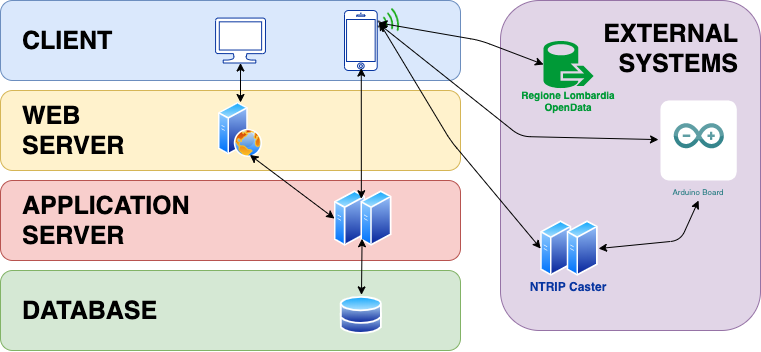
\includegraphics[width=\textwidth]{img/archi/layers.png}
  \hspace{0.05\linewidth}
  \centering
  \caption{\textit{Layered Structure} of the system}
  \label{img:archi_layers}
\end{center}
\end{figure}
\clearpage

The considered high-level components are:
\customParagraph{Mobile Application} 
The \textit{Presentation Layer} dedicated to mobile devices. It communicates with the Application Server to retrieve and send data measured by the \textit{Arduino} board. It contains a wide part of the \textit{Logic Layer} to render data in different ways.\\
The communication with the \textit{Arduino} board is handled with the phone hotspot service; moreover, \textit{Arduino} board could retrieve the RTK GPS correction with a TCP connection with the NTRIPCaster.
  
\customParagraph{Web Browsers}
The \textit{Presentation Layer} dedicated to web browsers; it communicates directly with the Web Server.
  
\customParagraph{Web Server}
It communicates with the Application Server and with the Web Browsers. This is the layer that provides web-pages for the Web Browser; currently, it provides only the SwaggerUI documentation of the RestfulAPI.
  
\customParagraph{Application Server}
This is the layer in which is contained a part of the \textit{Logic Layer} to manage and store users information and collected data with the board; it communicates directly with the Mobile Application, the Web Server and the Database.
  
\customParagraph{Database}
The \textit{Data Layer} of the system; it includes all structures and entities responsible for data storage and management. It communicates with the Application Server.\\\\

In the Figure \ref{img:archi_layers}, \textit{Web Server} and \textit{Application Server} are separated because they represent different function of the application.\\
As mentioned before, it is not implemented a \textit{Web Application} on the \textit{Web Server}, so, in the current setting they are merged.\\ If in future a \textit{Web Application} will be implemented it could be useful to separate the two services in order to allow greater scalability.
\clearpage

\section{Component View}
In this section the system will be described in term of its components:  their functionalities will be discussed and detailed.\\
Moreover, interfaces among components and among external systems will be shown.

\subsection{Database}
The application database is managed using a Relational DBMS. \\
It allows the reading of data, ensuring to the users the possibility to log in, access the application of interest and check the stored data.
It is also used for data manipulation (insertion, modification and deletion).
The use of a Relational DBMS guarantees the fundamental properties for a database of this type:
\begin{itemize}
  \item \textit{Atomicity}: no partial executions of operations;
  \item \textit{Consistency}: the database is always in a consistent state;
  \item \textit{Isolation}: each transaction is executed in an isolated and independent way;
  \item \textit{Durability / Persistence}: changes made are not lost.
\end{itemize}

The database offers to the Application Server an interface that it can use to interact with it.
Particular attention must be paid to the encryption of passwords used to the user access to the system.
Below is the designed E-R diagram (Figure \ref{img:archi_er}).

\begin{figure}[H]
\begin{center}
  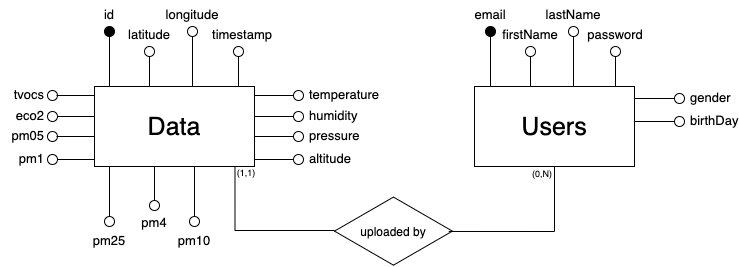
\includegraphics[width=\textwidth]{img/archi/ER.png}
  \hspace{0.05\linewidth}
  \centering
  \caption{\textit{Entity-Relationship} Diagram of the Database}
  \label{img:archi_er}
\end{center}
\end{figure}

\subsection{Application Server}
The main feature of the \textit{Application Server} is to define rules and work-flows of all the functionalities defined by the RestfulAPI.\\
The \textit{Application Server} must have interfaces to communicate with the \textit{Mobile Application} and also with the DBMS; the communication must be done through HTTPS protocol.\\
In the brief introduction below, logic modules and their descriptions are presented, while all the connections among them can be seen in the \textit{Global Component View} in Figure \ref{img:archi_components}.

\customParagraph{Authentication Service}
This module handles the authentication and authorization process. It generates authorization tokens and checks their validity.

\customParagraph{Arduino Data Controller}
This module receives the requests at the \textit{Arduino Data} endpoint, it checks the authorization using the interface with the \textit{Authentication Service} and pass them to the \textit{Arduino Data Service}.

\customParagraph{Arduino Data Service}
This module manages the requests for \textit{Arduino Data} interfacing itself with the \textit{Data Service}.

\customParagraph{Data Service}
This module is the unique interface of the \textit{Application Server} to the database's DBMS.

\customParagraph{User Controller}
This module receives the requests at the \textit{User} endpoint, it checks the authorization using the interface with the \textit{Authentication Service} and pass them to the \textit{User Service}.

\customParagraph{User Service}
This module manages the requests for a \textit{User} interfacing itself with the \textit{Data Service}.

\clearpage
\subsection{Web Server}
As already explained before, the \textit{Web Server} is a simple service. It provides a simple web-page to redirect the user to the \textit{SwaggerUI} documentation.\\
The \textit{Web Server} is hosted in the same space of the \textit{Application Server}; so the connections are done with the HTTPS protocol.\\

\subsection{Mobile Application}
The \textit{MOQA} mobile application communicates with the \textit{Application Server} through RestfulAPIs that are defined in order to describe the interactions between the two layers and that must be independent from the two implementations.\\
The application manages the connection with the \textit{Arduino} board to get air and weather measures and send these data to the \textit{Application Server}. Moreover, it manages the connection with the \textit{Regione Lombardia OpenData} service to retrieve ARPA data.\\

The detailed behaviour of the components in the mobile application is discussed in the Section \ref{sec:ci_mobile}.

\begin{figure}[H]
\begin{center}
  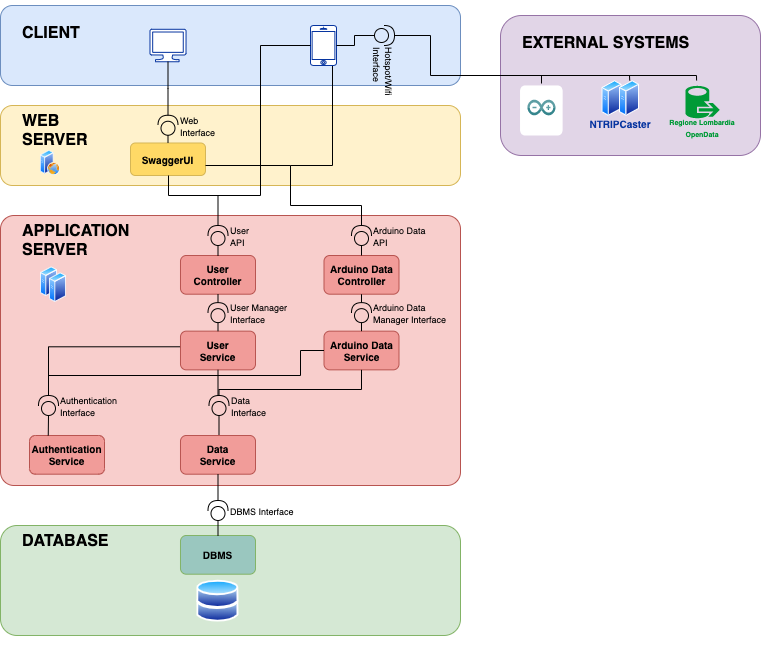
\includegraphics[width=\textwidth]{img/archi/components.png}
  \hspace{0.05\linewidth}
  \centering
  \caption{\textit{Global Component View}}
  \label{img:archi_components}
\end{center}
\end{figure}
\clearpage

\section{Deployment View}
Below is the deployment diagram of the system (Figure \ref{img:archi_deployment}).

\begin{figure}[H]
\begin{center}
  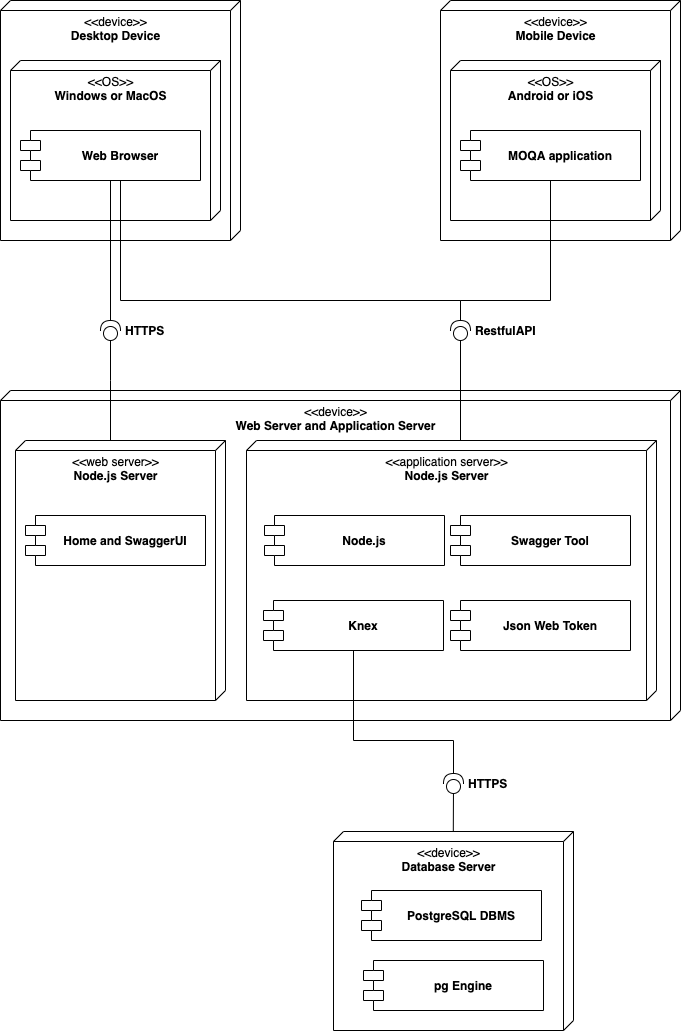
\includegraphics[width=\textwidth,height=.83\textheight,keepaspectratio]{img/archi/deployment.png}
  \hspace{0.05\linewidth}
  \centering
  \caption{\textit{Deployment Diagram} of the system}
  \label{img:archi_deployment}
\end{center}
\end{figure}

\section{Runtime View}\label{sec:runtime}
The aim of this section is to specify the behaviour of the system. Some relevant cases are selected and exploit using \textit{Sequence Diagrams}.

\begin{figure}[H]
\begin{center}
  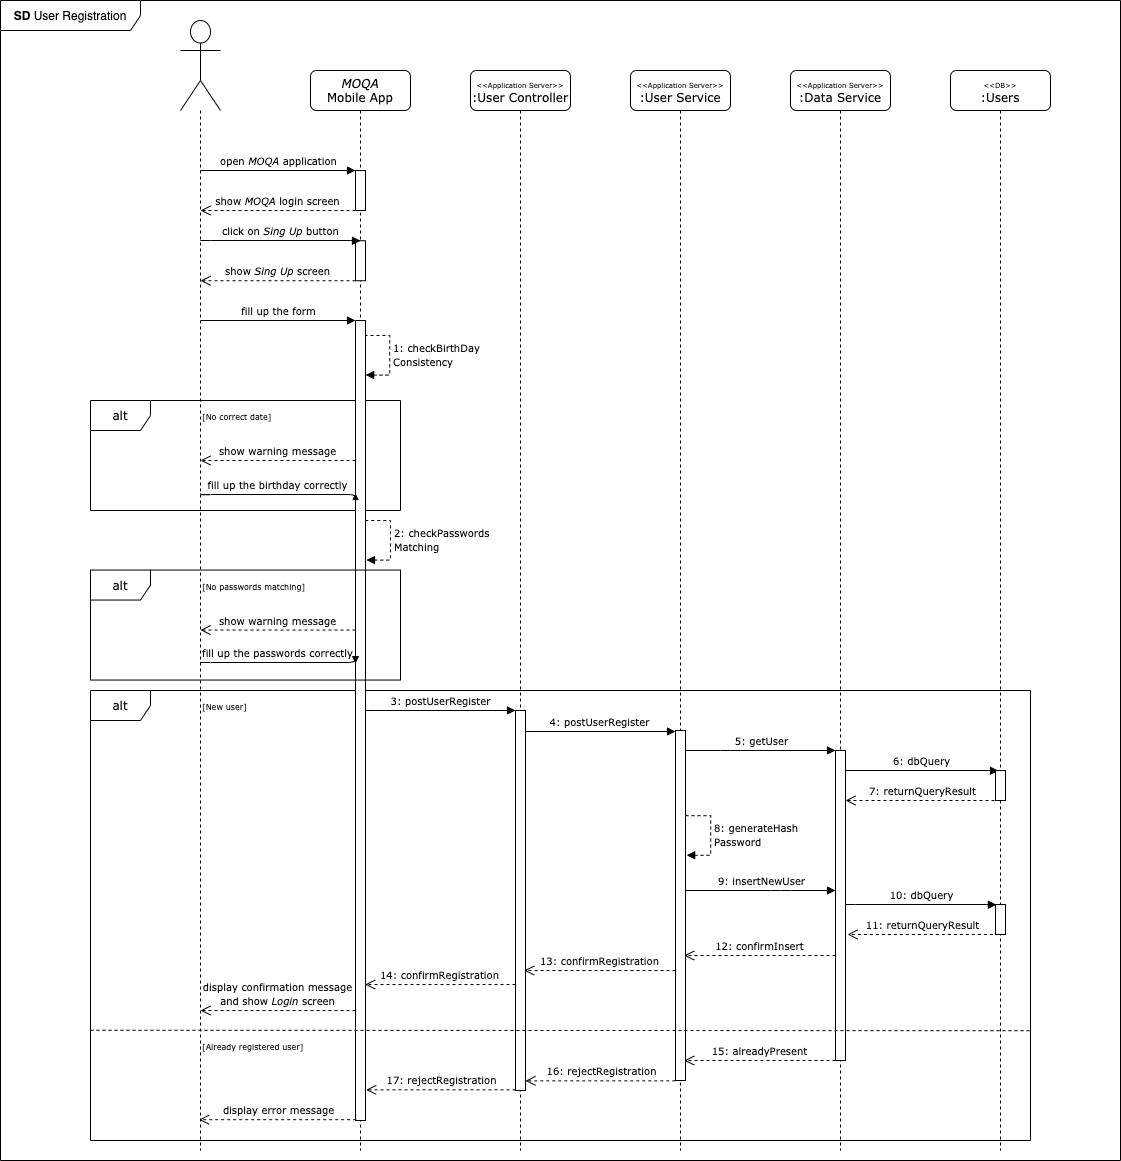
\includegraphics[width=\textwidth,keepaspectratio]{img/archi/sequences/signup.png}
  \hspace{0.05\linewidth}
  \centering
  \caption{\textit{User Signup} sequence diagram: it describes the process through which a user can register itself in the system}
  \label{img:archi_er}
\end{center}
\end{figure}






\section{Component Interfaces}
This section contains some detailed information about the interfaces between the components of the system.\\
The following description focuses the attention over the actions performed by a procedure of a certain component after that it is called by other components.\\
Huge part of these actions could be seen played in the \textit{Sequence Diagrams} (Section \ref{sec:runtime}).

\subsection{Application Server}

\customParagraph{Authentication Service}
Following procedures are called by other components:
\begin{itemize}
    \item \textbf{generateJWT}\quad This method allows to generate a token for the authentication. The token must be added in the requests as \textit{Header} attribute.
    \item \textbf{decodeJWT}\quad This method allows to get and decode the token, if present, in a request. It returns the object with the information of the.
\end{itemize}

\customParagraph{Arduino Data Controller}
Following procedures are called by other components:
\begin{itemize}
    \item \textbf{getData}\quad This method is called when a request is received at the corresponding endpoint. It calls the \textit{Authentication Service} to check the session. If the session is valid, it retrieves the parameters in the request and calls the corresponding method in the \textit{Arduino Data Service}.
    \item \textbf{getDataByDate}\quad This method is called when a request is received at the corresponding endpoint. It calls the \textit{Authentication Service} to check the session. If the session is valid, it retrieves the parameters in the request and calls the corresponding method in the \textit{Arduino Data Service}.
    \item \textbf{postData}\quad This method is called when a request is received at the corresponding endpoint. It calls the \textit{Authentication Service} to check the session. If the session is valid, it retrieves the parameters in the request and calls the corresponding method in the \textit{Arduino Data Service}.
\end{itemize}

\customParagraph{Arduino Data Service}
Following procedures are called by other components:
\begin{itemize}
    \item \textbf{getData}\quad This method is called by the \textit{Arduino Data Controller}. It retrieves the data preparing the query to submit to the \textit{Data Service}.
    \item \textbf{getDataByDate}\quad This method is called by the \textit{Arduino Data Controller}. It retrieves the data preparing the query to submit to the \textit{Data Service}
    \item \textbf{postData}\quad This method is called by the \textit{Arduino Data Controller}. It retrieves the data preparing the query to submit to the \textit{Data Service}
\end{itemize}

\customParagraph{Data Service}
Following procedure is called by other components:
\begin{itemize}
    \item \textbf{databaseInit}\quad This method is called during the initialization of the \textit{Application Server} to create the tables in the database and initialize them with the initials data.
\end{itemize}

Moreover, it provides an object that has own methods to query the database through the DBMS service.

\customParagraph{User Controller}
Following procedures are called by other components:
\begin{itemize}
    \item \textbf{deleteUserMe}\quad This method is called when a request is received at the corresponding endpoint. It calls the \textit{Authentication Service} to check the session, if the session is valid it retrieves, from the session, the user email and calls the corresponding method in the \textit{Arduino Data Service}.
    \item \textbf{getUserMe}\quad This method is called when a request is received at the corresponding endpoint. It calls the \textit{Authentication Service} to check the session, if the session is valid it retrieves, from the session, the user email and calls the corresponding method in the \textit{Arduino Data Service}.
    \item \textbf{postUserLogin}\quad This method is called when a request is received at the corresponding endpoint. It retrieves the parameters in the request and calls the corresponding method in the \textit{Arduino Data Service}.
    \item \textbf{postUserLogout}\quad This method is called when a request is received at the corresponding endpoint. It calls the \textit{Authentication Service} to check the session, if the session is valid it logout the user.
    \item \textbf{postUserRegister}\quad This method is called when a request is received at the corresponding endpoint. It retrieves the parameters in the request and calls the corresponding method in the \textit{Arduino Data Service}.
    \item \textbf{putUserMe}\quad This method is called when a request is received at the corresponding endpoint. It calls the \textit{Authentication Service} to check the session. If the session is valid, it retrieves the parameters in the request, checks the consistency* and calls the corresponding method in the \textit{Arduino Data Service}.
\end{itemize}

*: the consistency is computed checking if the session email is the same in the body in the PUT request.

\customParagraph{User Service}
Following procedures are called by other components:
\begin{itemize}
    \item \textbf{deleteUserMe}\quad This method is called by the \textit{User Controller}. It retrieves the data preparing the query to submit to the \textit{Data Service}.
    \item \textbf{getUserMe}\quad This method is called by the \textit{User Controller}. It retrieves the data preparing the query to submit to the \textit{Data Service}.
    \item \textbf{postUserLogin}\quad This method is called by the \textit{User Controller}. It retrieves the data preparing the query to submit to the \textit{Data Service}.
    \item \textbf{postUserRegister}\quad This method is called by the \textit{User Controller}. It retrieves the data preparing the query to submit to the \textit{Data Service}.
    \item \textbf{putUserMe}\quad This method is called by the \textit{User Controller}. It retrieves the data preparing the query to submit to the \textit{Data Service}.
\end{itemize}

\subsection{Mobile Application}\label{sec:ci_mobile}


\section{Architecture styles and patterns}